% background chapter continued
\section{Mercator Architecture}\index{Mercator Architecture}
to use its 'blueprint-design'

\begin{figure}[h!]
  \centering
  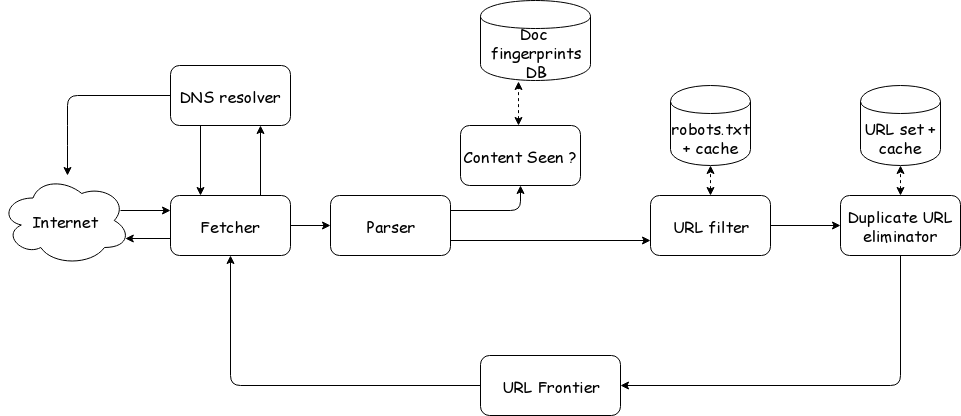
\includegraphics[width=15cm,height=12cm,keepaspectratio]{../media/crawler/basic-crawler-architecture-v2.png}
  \caption{Crawler architecture}
  \label{fig:basicarch}
\end{figure}

\subsection{Fetcher, Parser, and DNS}\index{Fetcher, Parser, and DNS}
\subsection{Handling De-duplication}\index{Handling De-duplication}
\subsection{URL Filtering}\index{URL Filtering}
\subsection{Duplicate URL Eliminator (DUE)}\index{Duplicate URL Eliminator(DUE)}

\pagebreak

\subsection{URL Frontier}
some text here
\begin{figure}[h!]
  \centering
  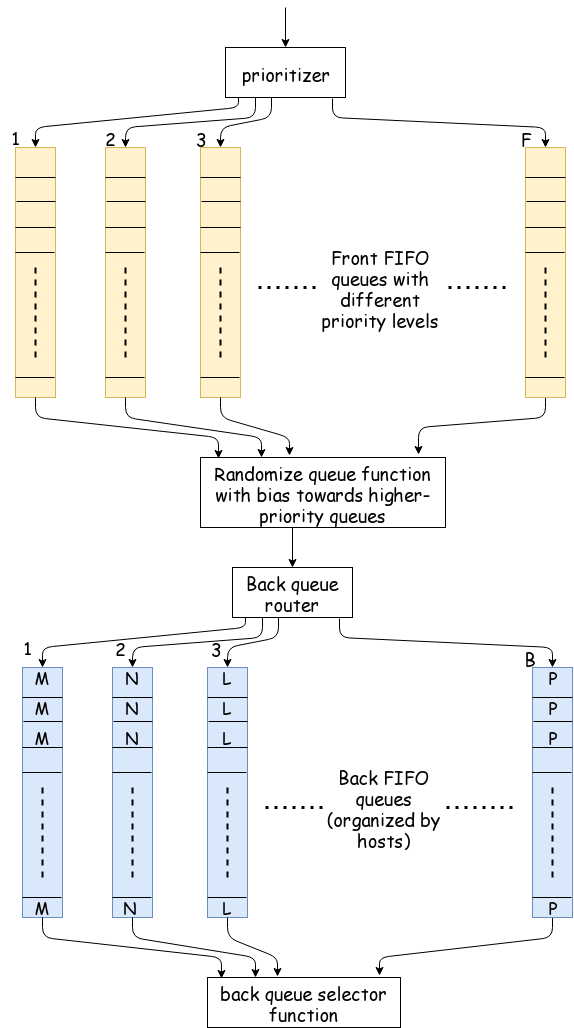
\includegraphics[width=10cm,height=13cm,keepaspectratio]{../media/crawler/url-frontier.png}
  \caption{URL Frontier Scheme(based on Mercator)}
  \label{fig:frontier}
\end{figure}

\pagebreak
some text here
\begin{figure}[h!]
  \centering
  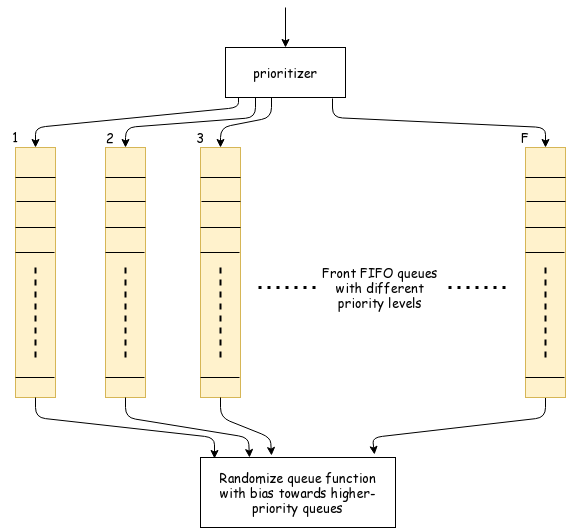
\includegraphics[width=13cm,height=10cm,keepaspectratio]{../media/crawler/f-queue.png}
  \caption{Frontier Front Queue}
  \label{fig:fqueue}
\end{figure}

\pagebreak
some text here
\begin{figure}[h!]
  \centering
  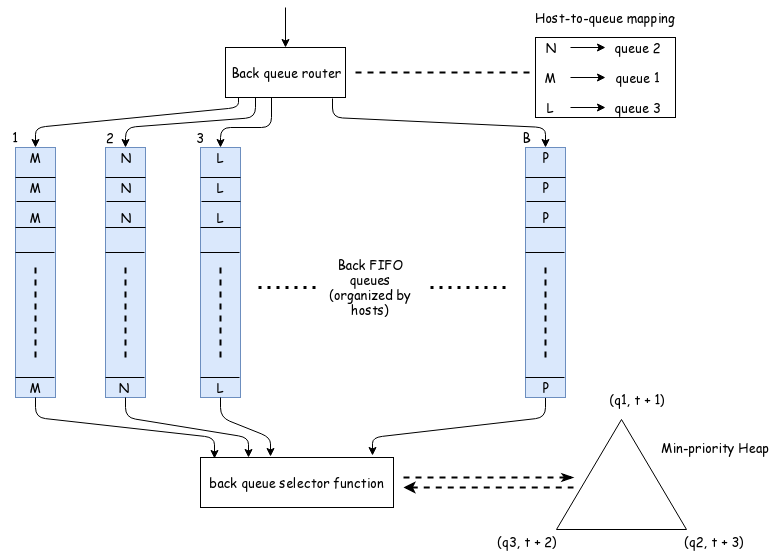
\includegraphics[width=13cm,height=10cm,keepaspectratio]{../media/crawler/b-queue.png}
  \caption{Frontier Back Queue}
  \label{fig:bqueue}
\end{figure}

\pagebreak
some text here
\subsection{Distributing Web Crawl}\index{Distributing Web Crawl}
\begin{figure}[h!]
  \centering
  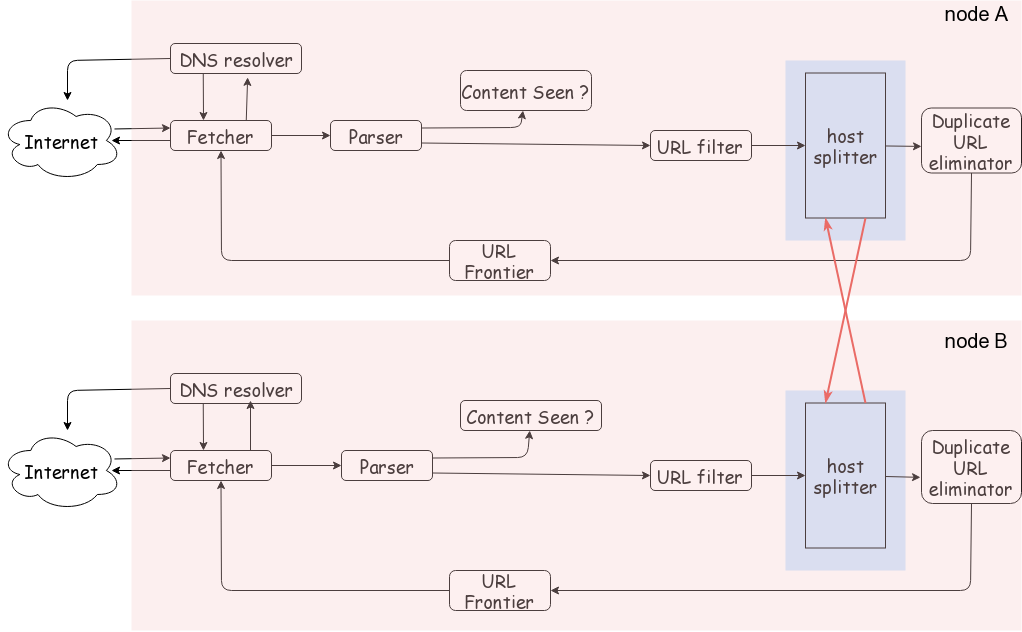
\includegraphics[width=15cm,height=10cm,keepaspectratio]{../media/crawler/host-splitterv3.png}
  \caption{Host Partitioning}
  \label{fig:hpart}
\end{figure}

\pagebreak

\section{Automata Analogy}\index{Automata Analogy}